%
% LATEXBONES
%
\documentclass[a4paper,11pt,twoside]{article}
\usepackage{graphicx}
\usepackage{amsmath}
\usepackage[english]{babel}
\usepackage[applemac]{inputenc}
\usepackage[colorlinks,bookmarks=false,linkcolor=blue,urlcolor=blue]{hyperref}
\usepackage{subfigure}
\usepackage{here}
\usepackage{wrapfig}
\usepackage{fancyhdr}
%\usepackage{dirtytalk}

%drow graph
\usepackage{fancybox}
\usepackage{tikz}
\usepackage{capt-of}

% print code
\usepackage{listings}
\usepackage{algorithm2e}
\usepackage{verbatim}

% push at the bottom
\newenvironment{bottompar}{\par\vspace*{\fill}}{\clearpage}

% landscape
\usepackage{pdflscape}

\paperheight=297mm
\paperwidth=210mm

\setlength{\textheight}{235mm}
\setlength{\topmargin}{-1.2cm} 

\setlength{\parindent}{0pt}

\setlength{\textwidth}{15cm}
\setlength{\oddsidemargin}{0.56cm}
\setlength{\evensidemargin}{0.56cm}

% quotes
\usepackage{framed}
\newcommand*{\signed}[1]{%
  \unskip\hspace*{1em plus 1fill}%
  \nolinebreak[3]\hspace*{\fill}\mbox{#1}
}

\pagestyle{plain}

% multiline equation -- call it with \begin{multline}
\usepackage{amsmath}


% --- equations ---
\def \be {\begin{equation}}
\def \ee {\end{equation}}
%\def \dd  {{\rm d}}m

% --- links ---
\newcommand{\mail}[1]{{\href{mailto:#1}{#1}}}
\newcommand{\ftplink}[1]{{\href{ftp://#1}{#1}}}







% ======= Document ======

%----------------------------------------------------------------------------------------
% HEADING SECTIONS
%----------------------------------------------------------------------------------------

% --- header ---
\fancyhead[L]{Discounting and valuation}
\fancyhead[R]{}

% no newpage after title
\let\endtitlepage\relax

% no enumeration of sections
\setcounter{secnumdepth}{0}

\begin{document}
\begin{titlepage} %Titre
\begin{center}
\newcommand{\HRule}{\rule{\linewidth}{0.5mm}} % Defines a new command for the horizontal lines, change thickness here
\center % Center everything on the page
 
 
 %----------------------------------------------------------------------------------------
% TITLE SECTION
%----------------------------------------------------------------------------------------




\begin{figure} [h] %----------- SubGraph ---------------------
\centerline{
\subfigure{
\includegraphics[height = 2 cm]{./pic/EPFL.png}  }
} 
\end{figure}

\HRule \\[0.4cm]
{ \huge \bfseries MGT-482 Principles of Finance \\Assignment 5}\\[0.4cm] % Title of your document

\begin{minipage}[t]{0.4\textwidth}
\flushleft
Prof. Erwan Morellec
\end{minipage}
~
\begin{minipage}[t]{0.55\textwidth}
\flushright
Team: \\
Joachim Muth - \mail{joachim.muth@epfl.ch}\\
Andreas Bill - \mail{andreas.bill@epfl.ch}\\
Nicolas Roth - \mail{nicolas.roth@epfl.ch}\\
\end{minipage}
\begin{center}
\today
\end{center}
\HRule \\
 %----------------------------------------------------------------------------------------

\end{center}
\end{titlepage}



\pagestyle{fancy}
% ================ Introduction ==============
% ================ Ex 1 ==============
\section{Exercice 1}

\subsection{Solution to a.)}
We can compute the Sharpe ratio of a portfolio by applying equation \ref{eq1}:

\begin{equation}
\label{eq1}
\text{Sharp ratio} = \frac{\text{Portfolio excess return}}{\text{Portfolio volatility}} = \frac{E[R_p]-r_f}{SD(R_p)}
\end{equation}

For the portfolio with the given caracteristics, this resolves to: $\frac{12\% - 5\%}{10\%} = 0.7$

\subsection{Solution to b.)}

The CML is the straight line starting at the risk-free rate of interest and passing through the efficient portfolio. The equation of the line is therefore given by $m*SD(R)+b$ where b ist the risk-free interest rate and m the slope of the CML which can be computed as $\frac{E[R_{Mkt}]-r_f}{SD(R_{Mkt})} = \frac{17\%-5\%}{12\%} = 1$. The equaion for the CML is therefore $0.05+SD(R)$.

\subsection{Solution to c.)}

We can compute the maximal expected return for a given CML by just inserting the volatility value into the CML equation. Therefore we get: $E[R_{max}] = 0.05+0.1 = 15\%$. As we have invested 250'000\$, the maximum expected return in \$ is $0.15*250'000 = 37'500\$ $.


% ================ Ex 2 ==============
\section{Exercice 2}

For this exercice we can compute the equation for the CML first and use it in order to find the wanted values. We know the intercept with the y-axis to be $r_f = 5\%$, and can compute the slope as in the previous exercice: $\frac{E[R_{Mkt}]-r_f}{SD(R_{Mkt})} = \frac{10\%-5\%}{18\%} = 0.2\overline{7}$. So the CML equation is: $E[R_p] = 0.05+2.\overline{7}*SD(R_p)$.

\subsection{Solution for a.)}

We want the expected return to be the same as in the original portfolio but have the lowest possible volatility for such a return. We need to determine how much we have to invest in the market portfolio in order to get the same expected return than in the original portfolio. We use equation \ref{eq2}:

\begin{equation}
\label{eq2}
E[R_{xCML}] = r_f + x*(E[R_{Mkt}] -r_f)
\end{equation}

Now we need to solve for x when $E[R_{xCML}] = E[R_O] = 12\% $. We get: \\ $x = \frac{E[R_{xCML}]-r_f}{E[R_{Mkt}] -r_f} = \frac{12\% - 5\%}{10\% - 5\%} = 1.4$ \\

So in order to get the same expected return with the lowest possible volatility we sell the Microsoft stock, add or borrow an additionnal $40\% = 0.4*15'000\$ = 6'000\$ $ and invest 21'000\$ in the market portfolio. The associated volatility of this investment is $1.4*SD(R_{Mkt}) = 1.4*18\% = 25.2\% $. We could also have gotten this value by solving the CML equation for an expected return of 12\%.

\subsection{Solution for b.)}
We can compute the highest possible expected return by inserting the volatility value of the Microsoft portfolio into the CML equation: $ E[R_p] = 0.05+0.2\overline{7}*0.4 = 16.\overline{1}\% $. So the highest expected return for a volatility of $40\%$ is $16.\overline{1}\% $. Now if we want to know how much we have to invest in the market porftolio to get this expected return we can compute x from \ref{eq2} as we did in the previous exercice: \\
$x = \frac{E[R_{xCML}]-r_f}{E[R_{Mkt}] -r_f} = \frac{16.\overline{1}\% - 5\%}{10\% - 5\%} = 2.\overline{2}$ \\ The alternative investment which has the highest expected return for the same volatility level is to add or borrow $1.\overline{2} * 15'000\$ = 18'333.\overline{3}\$ $ and invest $33'333.\overline{3}\$ $ in the market portfolio.



% ================ Ex 3 ==============
\section{Exercice 3}

\subsection{Solution for a.)}

From the Two-fund separation theorem we know that all investors will invest in the same tangent portfolio. Indeed, we can see that the weights of the two risky securities A and B are the same for both portfolio managers: $w_A = \frac{4'000+6'000}{4'000} = \frac{2'500+3'750}{2'500} = 0.4$ and because there are only two possible assets: $w_B = 1-w_A = 0.6$. The composition of the tangency portfolio is therefore 0.4*A + 0.6*B. The volatility of the tangency portfolio can be computed using equation \ref{eq3} which simplifies to equation \ref{eq4} as the correlation of the two assets is 0. The expected return using equation \ref{eq5}. 

\begin{equation}
\label{eq3}
Var(R_p) = x_1^2*SD(R_1)^2+x_2^2+SD(R_2)^2 + 2*x_1*x_2*Corr(R_1,R_2)*SD(R_1)*SD(R_2) 
\end{equation}

\begin{equation}
\begin{split}
\label{eq4}
Var(R_p) = x_1^2*SD(R_1)^2+x_2^2+SD(R_2)^2 = 0.4^2*0.09 + 0.6^2*0.15 = 0.0684 \\
SD(R_p) = \sqrt{Var(R_p)} = \sqrt{0.0684} = 26.15\%
\end{split}
\end{equation}

\begin{equation}
\label{eq5}
R_p = x_1*R_1+x_2*R_2 = 0.4*0.05+0.6*0.08 = 0.068 = 6.8\%
\end{equation}

\subsection{Solution for b.)}

Portfolio manager 2 does not need to change his portfolio as he didn't borrow in the first place. However portfolio manager 1 will not be able to borrow money now, so he will only be able to invest 8'000\$ instead of the 10'000\$ he had invested before. He will invest these 8'000\$ according to the composition of the tangency portfolio determined before, namely 3'200\$ in security A and 4'800 in security B. His expected return as well as the volatility will be reduced to those of the tangency portfolio described in subproblem a. Figure \ref{fig1} shows the location of the two portfolios on the CML before and after the new regulation.

\begin{figure}[h!]
\center
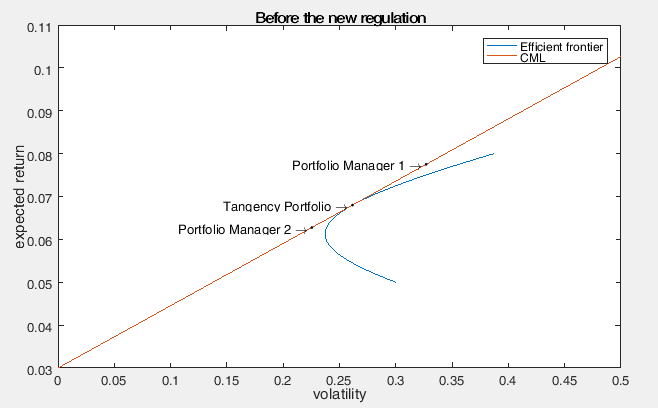
\includegraphics[width = .9 \linewidth]{Before.png}

\vspace{10pt}

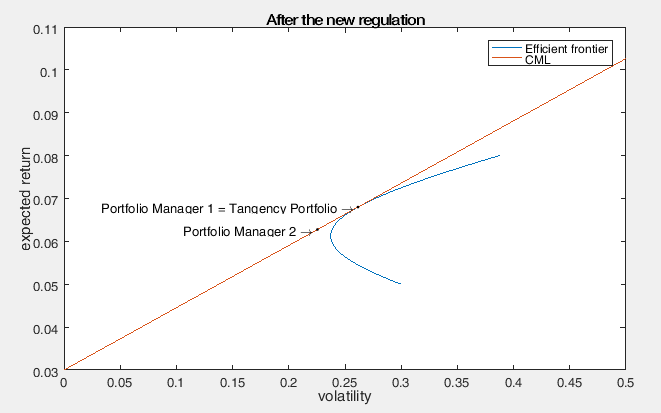
\includegraphics[width = .9 \linewidth]{After.png}
\caption{Investments of the two portfolio managers}
\label{fig1}
\end{figure}

% ================ Ex 4 ==============
\section{Exercice 4}

The return of a portfolio is given by the weighted average of the returns of each asset. The shortsell of XYZ industries can be seen as a negative investment in XYZ industries. Therefore we need to compute the return of the following portfolio:

\begin{center} %---------------Tab--------------
\begin{tabular} { c  c  c  c }
Asset & Investment & weight  & return \\[5pt]
\hline \\[-5pt]
US treasury bills & 37'500 & $ \frac{37'500}{-12'500+37'500} = 1.5 $ & 5\% \\[5pt]
\hline \\[-5pt]
XYZ Industries & -12'500 & $ \frac{-12'500}{-12'500+37'500} = -0.5 $ & ? \\[5pt]
\hline
\end{tabular}
\end{center}

In order to calculate the return on this portfolio we need to know the return of XYZ Industries. This is computed by equation \ref{eq6}:

\begin{equation}
\label{eq6}
R_{t+1} = \frac{Div_{t+1} + P_{t+1}}{P_t} - 1 = \frac{2.5 + 72.5}{62.5} - 1 = 20\% 
\end{equation}

Now we just need to do the weighted mean: 

\begin{equation}
\label{eq7}
R_p = 1.5*0.05-0.5*0.2 = -0.025 = -2.5\%
\end{equation}


% ================ Ex 5 ==============
\section{Exercice 5}

\subsection{Solution for a.)}
Under the CAPM relation, equation \ref{eq8} is used in order to calculate the expected return of an asset which is correlated with the market.

\begin{equation}
\label{eq8}
E[R_i] = r_i = r_f + \beta_i^{Mkt}*(E[R_{Mkt}]-r_f)
\end{equation}

Before we can apply equation \ref{eq8} we need to compute the beta of each asset. This is done applying equation \ref{eq9}

\begin{equation}
\label{eq9}
\beta_i^{Mkt} = \frac{SD(R_i)*Corr(R_i,R_{Mkt})}{SD(R_{Mkt})}
\end{equation}

Inserting the volatility and market correlation values from the exercice into equation \ref{eq9} and then compute equation \ref{eq8}, we get the following betas and expected returns on the three stocks:

\begin{center} %---------------Tab--------------
\begin{tabular} { c  c  c}
Stock & Beta & Expected return\\[5pt]
\hline \\[-5pt]
A & 0.48 & 5.88\% \\[5pt]
\hline \\[-5pt]
B & 1.2 & 10.2\% \\[5pt]
\hline \\[-5pt]
C & -0.18 & 1.92\%\\[5pt]
\hline
\end{tabular}
\end{center}

\subsection{Solution for b.)}

The expected return of a portfolio is the weighted average of the expected returns of its assets. We get: $0.6*0.0588+0.3*0.102+0.1*0.0192 = 0.0678 = 6.78\% $

\subsection{Solution for c.)}

The beta of a portfolio is the weighted average of the betas of its assets:\\ $0.6*0.48 + 0.3*1.2 +0.1*(-0.18) = 0.63$

\subsection{Solution for d.)}

We apply equation \ref{eq10} in order to compute the idiosyncratic risk ($\sigma_\epsilon$ of a stock:

\begin{equation}
\label{eq10}
\sigma_i^2 = \beta_i^2*\sigma_{Mkt}^2+\sigma_\epsilon^2 \rightarrow \sigma_\epsilon = \sqrt{\sigma_i^2-\beta_i^2*\sigma_{Mkt}^2}
\end{equation}

The following table shows the results:

\begin{center} %---------------Tab--------------
\begin{tabular} { c  c  c  c }
Stock & $\beta$ & $\sigma$ & $\sigma_\epsilon$ \\[5pt]
\hline \\[-5pt]
A & 0.48 & 0.06 & 0.036 \\[5pt]
\hline \\[-5pt]
B & 1.2 & 0.4 & 0.382\\[5pt]
\hline \\[-5pt]
C & -0.18 & 0.09 & 0.088 \\[5pt]
\hline
\end{tabular}
\end{center}

\subsection{Solution for e.)}
We can write the total risk (volatility) of the portfolio is the sum of systematic- and idiosyncratic risk.\\ Systematic risk can be written as: $\sigma_{syst,P} = \beta_P*\sigma_{Mkt} = 0.63*0.1 = 6.3\%$. \\
Idiosyncratic risk of a portfolio is: $\sigma_{\epsilon,P} = \sqrt{\sum_{i=1}^3w_i^2*\sigma_i^2}$, using the weights and volatility values from the exercice we get: \\[5pt] $\sqrt{0.6^2*0.06^2+0.3^2*0.4^2+0.1^2*0.09^2} = 0.1256 = 12.56\%$. \\[5pt]
Now we can compute the total volatility using equation \ref{eq10}: \\[5pt]
$\sigma_P = \sqrt{\beta_P^2*\sigma_{Mkt}^2+\sigma_{\epsilon,P}^2} = \sqrt{0.63^2*0.1^2+0.1256^2} = 14.05\% $
% ================ Ex 6 ==============
\section{Exercice 6}

We compute the beta using equation \ref{eq9}: \\[5pt]$\beta_{M\&Co} = \frac{SD(R_{M\&Co})*Corr(R_{M\&Co},R_{Mkt})}{SD(R_{Mkt})} = \frac{0.2*0.06}{0.16} = 0.075$ \\[5pt]
The expected return on Merck\&Co can now be computed using equation \ref{eq8}: \\
$E[R_{M\&Co}] = r_f + \beta_{M\&Co}^{Mkt}*(E[R_{Mkt}]-r_f) = 0.04+0.075*(0.1-0.04) = 4.45\%$ \\[5pt]

% ================ Ex 7 ==============
\section{Exercice 7}
\subsection{Solution for a.)}
In order to apply equation \ref{eq8} for the calculation of the expected return of A, we first need to compute the expected return of the market. We can do this based on the information we have about B: \\[5pt]
$E[R_{B}] = r_f + \beta_B^{Mkt}*(E[R_{Mkt}]-r_f) \rightarrow E[R_{Mkt}] = \frac{E[R_B]-r_f}{\beta_B^{Mkt}} + r_f = \frac{0.08-0.02}{0.75}+0.02 = 10\%$\\[5pt]
Now we can apply equation \ref{eq8}: \\[5pt]
$E[R_A] = r_f + \beta_A^{Mkt}*(E[R_{Mkt}]-r_f) = 0.02+1.4*(0.1-0.02) = 13.2\% $\\[5pt]
The Beta of C is computed by rearranging equation \ref{eq8}: \\[5pt]
$E[R_C] = r_f + \beta_C^{Mkt}*(E[R_{Mkt}]-r_f) \rightarrow \beta_C = \frac{E[R_C]-r_f}{E[R_{Mkt}]-r_f} = \frac{0.15-0.02}{0.1-0.02} = 1.625$

\subsection{Solution for b.)}
The beta of the market portfolio is 1. This is obvious as the beta determines how much a portfolio moves with the market.

\subsection{Solution for c.)}
Well we know that the beta of a portfolio is the weighted sum of its assets. We can therefore write: $\beta_{Mkt} = x_A*beta_a + x_B*\beta_B + x_C*\beta_C$, and using the known values of all betas: $1 = x_A*1.4+x_B*0.75+x_C*1.625$. We also know that the weight of stock C ($x_C$) is one third of the weight of stock B ($x_B$). We can now write: $1 = x_A*1.4+x_B*0.75+\frac{x_B}{3}*1.625$. The sum of the weights has to be equal to 1 as well. So we have two equations with two unknowns: \\[10pt]
$x_A*1.4+x_B*0.75+\frac{x_B}{3}*1.625 = 1$ \\[5pt]
$x_A + \frac{4}{3}*x_B = 1$\\[10pt]

Solving this small system of equations leads to following solution for the composition of the market portfolio: \\[5pt]
$x_A = 7.2\%$\\
$x_B = 69.6\%$\\
$x_C = 23.2\%$\\



%======= TABLEAU ===========
%\begin{center} %---------------Tab--------------
%\begin{tabular} {| c | c | c | c | c | c |}
%\hline
 %& & & & & $\\ \hline
%\end{tabular}
%\end{center}


%===========GRAPH================
%\begin{figure} %---------------------Graph---------------------------
%\begin{center}
%\includegraphics[width=12cm]{graph/ampli2} 
%\end{center}
%\caption{\em  \label{label}
%L�gende
%}
%\end{figure}


%========SUBGRAPH=======
%\begin{figure} [h] %----------- SubGraph ---------------------
%\centerline{
%\subfigure[ sublegend ] {\label{sfig:thetat} \includegraphics[width=7cm]{ graph/graph_convdt3 } }
%\subfigure[ sublegend ] {\label{sfig:thetafin} \includegraphics[width=7cm]{ graph/graph_convtfin } } 
%}
%\caption{\label{ label } 
%L�gende
%} 
%\end{figure}








\end{document} %%%% THE END %%%%
